
\begin{center}
    \Large\textbf{Gradio: Biến Ý Tưởng Thành Giao Diện Chỉ Trong Vài Phút!}
\end{center}

\begin{center}
    \Large\textit{Đàm Nguyên Khánh}
\end{center}

\label{sec:gradio}

\begin{abstract}
Gradio là một thư viện Python mã nguồn mở được phát triển bởi Hugging Face, cho phép tạo giao diện web tương tác cho các mô hình Machine Learning chỉ trong vài dòng code. Bài viết này trình bày chi tiết về Gradio từ cơ bản đến nâng cao, bao gồm:

\textbf{Điểm nổi bật:}
\begin{itemize}
    \item \textbf{Tạo giao diện nhanh chóng}: Chỉ cần 5-10 dòng code để tạo demo ML hoàn chỉnh
    \item \textbf{Hỗ trợ đa dạng input/output}: Text, Image, Audio, Video, File, JSON với hơn 20 loại components
    \item \textbf{Tích hợp mạnh mẽ}: Hoạt động với TensorFlow, PyTorch, scikit-learn, XGBoost và hầu hết các framework ML
    \item \textbf{Deployment dễ dàng}: Từ local development đến production với Docker và cloud platforms
\end{itemize}

\textbf{Phạm vi ứng dụng:} Từ prototype đơn giản cho nghiên cứu đến ứng dụng production phức tạp với custom layout, event handling, và state management. Gradio phù hợp cho data scientists, ML engineers, và developers muốn demo nhanh ý tưởng ML.
\end{abstract}

\section{Giới thiệu Gradio}
\label{subsec:gradio-intro}

\begin{figure}[H]
    \centering
    \includegraphics[width=0.5\textwidth]{projects/Gradio Blog/image/gradio_logo.png}
    \caption{Logo chính thức của Gradio - Thư viện Python mã nguồn mở cho việc tạo giao diện web tương tác cho các mô hình Machine Learning.}
    \label{fig:gradio-logo}
\end{figure}

\subsection{Nguồn gốc và lịch sử phát triển}

Gradio ban đầu được phát triển bởi \textbf{Abubakar Abid} và nhóm \textbf{Gradio Labs} vào khoảng năm 2019. Mục tiêu ban đầu là tạo ra một thư viện giúp các nhà nghiên cứu và kỹ sư AI dễ dàng xây dựng giao diện web để demo mô hình Machine Learning chỉ bằng vài dòng Python.

Đến tháng 12/2021, \textbf{Hugging Face} đã mua lại Gradio. Kể từ đó, Gradio trở thành một phần quan trọng trong hệ sinh thái Hugging Face, được tích hợp chặt chẽ với \textbf{Hugging Face Spaces} để triển khai và chia sẻ demo AI trực tuyến.

\begin{tcolorbox}[colback=green!10,colframe=green!50!black,title=Lịch sử phát triển]
\begin{itemize}
    \item \textbf{2019}: Gradio Labs phát triển phiên bản đầu tiên
    \item \textbf{2021}: Hugging Face mua lại Gradio
    \item \textbf{2022-nay}: Tích hợp sâu với Hugging Face ecosystem
    \item \textbf{Hiện tại}: Hơn 1 triệu developers sử dụng, 500,000+ ứng dụng trên Spaces
\end{itemize}
\end{tcolorbox}

\subsection{Tổng quan về Gradio}

Gradio là một thư viện Python mã nguồn mở hiện được duy trì và phát triển bởi Hugging Face, cho phép tạo giao diện web tương tác cho các mô hình Machine Learning một cách nhanh chóng. Framework này đặc biệt hữu ích cho:

\begin{itemize}
    \item \textbf{Prototyping nhanh}: Tạo demo cho mô hình ML chỉ trong vài phút
    \item \textbf{Sharing và Collaboration}: Chia sẻ mô hình với đồng nghiệp và stakeholders
    \item \textbf{Testing và Validation}: Kiểm tra mô hình với dữ liệu thực tế
    \item \textbf{Production Deployment}: Triển khai ứng dụng ML lên web
\end{itemize}

\subsection{Ưu điểm của Gradio}

\begin{tcolorbox}[colback=green!10,colframe=green!50!black,title=Ưu điểm chính]
\begin{itemize}
    \item \textbf{Dễ sử dụng}: Chỉ cần vài dòng code để tạo giao diện
    \item \textbf{Linh hoạt}: Hỗ trợ nhiều loại input/output (text, image, audio, video)
    \item \textbf{Tích hợp tốt}: Hoạt động với mọi framework ML (TensorFlow, PyTorch, scikit-learn)
    \item \textbf{Responsive}: Giao diện tự động thích ứng với mọi thiết bị
    \item \textbf{Sharing}: Dễ dàng chia sẻ qua link public
\end{itemize}
\end{tcolorbox}

\subsection{Cài đặt Gradio}

\begin{minted}{bash}
# Cài đặt Gradio bằng pip (khuyến nghị)
pip install gradio

# Hoặc cài đặt bằng conda (cho môi trường conda)
conda install -c conda-forge gradio
\end{minted}

\textbf{Giải thích:}
\begin{itemize}
    \item \texttt{pip install gradio}: Cài đặt Gradio từ PyPI (Python Package Index) - cách phổ biến nhất
    \item \texttt{conda install -c conda-forge gradio}: Cài đặt qua conda từ channel conda-forge - phù hợp cho môi trường conda
    \item Sau khi cài đặt, bạn có thể import Gradio bằng \texttt{import gradio as gr}
\end{itemize}

\subsection{Kiến trúc Gradio}

\begin{figure}[H]
    \centering
    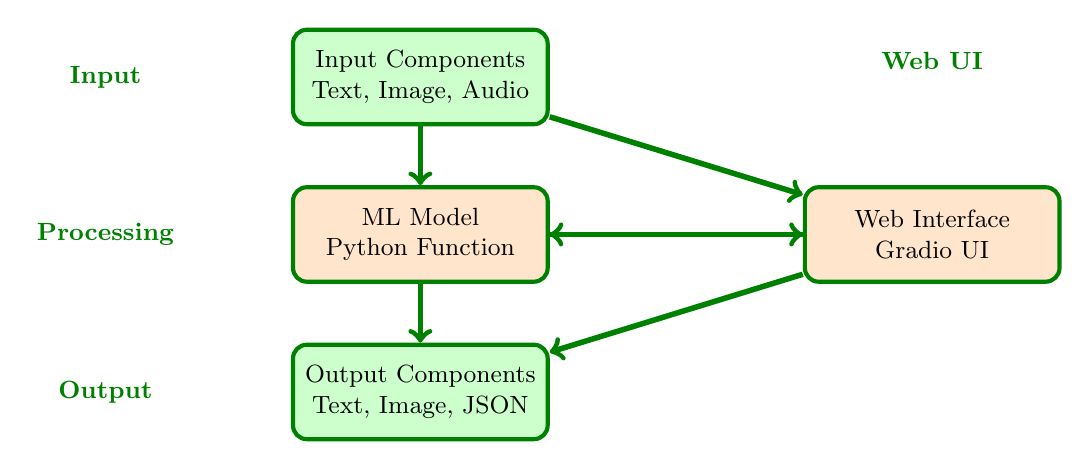
\begin{tikzpicture}[
        node distance=2.5cm,
        input/.style={rectangle, draw=green!50!black, fill=green!20, text width=3cm, text centered, minimum height=1.2cm, rounded corners=5pt, font=\small, line width=1.5pt},
        processing/.style={rectangle, draw=green!50!black, fill=orange!20, text width=3cm, text centered, minimum height=1.2cm, rounded corners=5pt, font=\small, line width=1.5pt},
        output/.style={rectangle, draw=green!50!black, fill=green!20, text width=3cm, text centered, minimum height=1.2cm, rounded corners=5pt, font=\small, line width=1.5pt},
        web/.style={rectangle, draw=green!50!black, fill=orange!20, text width=3cm, text centered, minimum height=1.2cm, rounded corners=5pt, font=\small, line width=1.5pt},
        arrow/.style={->, thick, green!50!black, line width=2pt},
        label/.style={font=\small\bfseries, green!50!black}
    ]
        % Input layer
        \node[input] (input) {Input Components\\Text, Image, Audio};
        
        % Processing layer
        \node[processing, below of=input, yshift=0.5cm] (processing) {ML Model\\Python Function};
        
        % Output layer
        \node[output, below of=processing, yshift=0.5cm] (output) {Output Components\\Text, Image, JSON};
        
        % Web interface
        \node[web, right of=processing, xshift=4cm] (web) {Web Interface\\Gradio UI};
        
        % Arrows
        \draw[arrow] (input) -- (processing);
        \draw[arrow] (processing) -- (output);
        \draw[arrow] (input) -- (web);
        \draw[arrow] (web) -- (processing);
        \draw[arrow] (processing) -- (web);
        \draw[arrow] (web) -- (output);
        
        % Labels
        \node[label, left of=input, xshift=-1.5cm] {Input};
        \node[label, left of=processing, xshift=-1.5cm] {Processing};
        \node[label, left of=output, xshift=-1.5cm] {Output};
        \node[label, above of=web, yshift=-0.3cm] {Web UI};
    \end{tikzpicture}
    \caption{Kiến trúc cơ bản của Gradio: Input components nhận dữ liệu từ người dùng, xử lý qua ML model hoặc Python function, và hiển thị kết quả qua output components. Web interface cung cấp giao diện tương tác cho toàn bộ quy trình.}
    \label{fig:gradio-architecture}
\end{figure}

\textbf{Giải thích chi tiết về kiến trúc:}
\begin{itemize}
    \item \textbf{Input Components} (Màu xanh lá): Các thành phần nhận dữ liệu đầu vào từ người dùng như Textbox, Image upload, Audio recorder, v.v.
    \item \textbf{ML Model/Python Function} (Màu cam): Trung tâm xử lý dữ liệu, có thể là mô hình Machine Learning hoặc function Python tùy chỉnh
    \item \textbf{Output Components} (Màu xanh lá): Các thành phần hiển thị kết quả như Text output, Image display, JSON data, v.v.
    \item \textbf{Web Interface} (Màu cam): Giao diện web tương tác được Gradio tự động tạo ra
    \item \textbf{Luồng dữ liệu}: Dữ liệu chảy từ Input → Processing → Output, với Web Interface làm cầu nối tương tác
\end{itemize}

\section{gr.Interface - Giao diện đơn giản}
\label{subsec:gradio-architecture}

\texttt{gr.Interface} là cách nhanh nhất để tạo giao diện web cho mô hình ML. Chỉ cần định nghĩa một hàm Python và cung cấp thông tin về input/output, Gradio sẽ tự động tạo ra giao diện web hoàn chỉnh. Phù hợp cho prototyping nhanh và demo đơn giản.

\subsection{Tạo ứng dụng đầu tiên}

\texttt{gr.Interface} là cách đơn giản nhất để bắt đầu với Gradio. Nó tự động tạo giao diện web dựa trên function Python của bạn, không cần kiến thức về HTML, CSS hay JavaScript. Gradio sẽ tự động xử lý routing, validation, và error handling.

Với \texttt{gr.Interface}, bạn có thể tạo giao diện web chỉ với vài dòng code:

\begin{minted}{python}
# Import thư viện Gradio
import gradio as gr

# Định nghĩa hàm xử lý dữ liệu
def greet(name):
    return "Hello, " + name

# Tạo giao diện Gradio
demo = gr.Interface(
    fn=greet,              # Hàm xử lý dữ liệu
    inputs=["text"],       # Loại input: text box
    outputs=["text"],      # Loại output: text box
)

# Khởi chạy ứng dụng web
demo.launch()
\end{minted}

\textbf{Giải thích từng dòng code:}
\begin{itemize}
    \item \texttt{import gradio as gr}: Import thư viện Gradio và đặt alias là \texttt{gr}
    \item \texttt{def greet(name):}: Định nghĩa hàm Python nhận tham số \texttt{name}
    \item \texttt{return "Hello, " + name}: Trả về chuỗi chào hỏi kết hợp với tên
    \item \texttt{gr.Interface()}: Tạo giao diện Gradio với các tham số:
    \begin{itemize}
        \item \texttt{fn=greet}: Chỉ định hàm xử lý dữ liệu
        \item \texttt{inputs=["text"]}: Tạo input text box
        \item \texttt{outputs=["text"]}: Tạo output text box
    \end{itemize}
    \item \texttt{demo.launch()}: Khởi chạy ứng dụng web trên localhost
\end{itemize}

\textbf{Kết quả:} Một ứng dụng web với input text box và output text box, khi người dùng nhập tên và nhấn Submit, sẽ hiển thị lời chào.

\subsection{Customizing Interface}

Gradio cung cấp nhiều tham số để tùy chỉnh giao diện, từ labels và placeholders đến themes và CSS. Các tham số này giúp tạo ra giao diện chuyên nghiệp và phù hợp với brand của bạn. Tất cả customizations đều được áp dụng real-time mà không cần restart server.

Bạn có thể tùy chỉnh giao diện với các tham số:

\begin{minted}{python}
# Tạo giao diện với các tùy chỉnh chi tiết
demo = gr.Interface(
    fn=greet,                                    # Hàm xử lý dữ liệu
    inputs=gr.Textbox(label="Enter your name",   # Input với label tùy chỉnh
                      placeholder="Type your name here..."),  # Placeholder text
    outputs=gr.Textbox(label="Greeting"),        # Output với label tùy chỉnh
    title="Greeting App",                        # Tiêu đề ứng dụng
    description="Enter your name to get a personalized greeting",  # Mô tả
    article="This is a simple demo of Gradio Interface"  # Thông tin bổ sung
)
\end{minted}

\textbf{Giải thích các tham số tùy chỉnh:}
\begin{itemize}
    \item \texttt{fn=greet}: Hàm xử lý dữ liệu (bắt buộc)
    \item \texttt{inputs=gr.Textbox(...)}: Tạo input text box với:
    \begin{itemize}
        \item \texttt{label}: Nhãn hiển thị bên trên input
        \item \texttt{placeholder}: Text gợi ý bên trong input box
    \end{itemize}
    \item \texttt{outputs=gr.Textbox(label="Greeting")}: Output text box với label
    \item \texttt{title}: Tiêu đề hiển thị ở đầu trang web
    \item \texttt{description}: Mô tả ngắn gọn về ứng dụng
    \item \texttt{article}: Thông tin bổ sung hiển thị ở cuối trang
\end{itemize}

\subsection{Các loại Input/Output}

Gradio hỗ trợ hơn 20 loại components khác nhau, từ text đơn giản đến file upload phức tạp. Mỗi component được tối ưu hóa cho các loại dữ liệu cụ thể và tự động xử lý validation, preprocessing, và error handling. Tất cả components đều responsive và hoạt động tốt trên mọi thiết bị.

Gradio hỗ trợ nhiều loại input/output:

\begin{itemize}
    \item \textbf{Text}: Văn bản đơn giản
    \item \textbf{Number}: Số liệu
    \item \textbf{Image}: Hình ảnh
    \item \textbf{Audio}: Âm thanh
    \item \textbf{Video}: Video
    \item \textbf{File}: File upload
    \item \textbf{Dataframe}: Bảng dữ liệu
    \item \textbf{JSON}: Dữ liệu JSON
\end{itemize}

\section{gr.Blocks - Giao diện phức tạp}
\label{subsec:gradio-interface-blocks}

\texttt{gr.Blocks} cung cấp khả năng tùy chỉnh cao cho các ứng dụng ML phức tạp. Với Blocks, bạn có thể tạo layout tùy chỉnh, xử lý nhiều events, quản lý state, và tích hợp nhiều functions. Phù hợp cho ứng dụng production và giao diện chuyên nghiệp.

Khi cần tạo giao diện phức tạp hơn, \texttt{gr.Blocks} là lựa chọn tốt nhất:

\begin{figure}[H]
\centering
    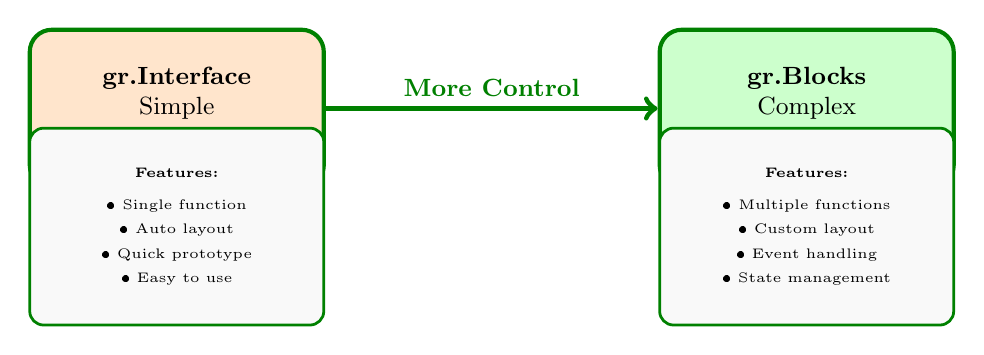
\begin{tikzpicture}[
        node distance=3cm,
        interface/.style={rectangle, draw=green!50!black, fill=orange!20, text width=3.5cm, text centered, minimum height=2cm, rounded corners=8pt, font=\small, line width=1.5pt},
        blocks/.style={rectangle, draw=green!50!black, fill=green!20, text width=3.5cm, text centered, minimum height=2cm, rounded corners=8pt, font=\small, line width=1.5pt},
        features/.style={rectangle, draw=green!50!black, fill=gray!5, text width=3.5cm, text centered, minimum height=2.5cm, rounded corners=5pt, font=\tiny, line width=1pt},
        arrow/.style={->, thick, green!50!black, line width=2pt},
        label/.style={font=\small\bfseries, green!50!black}
    ]
        % Interface
        \node[interface] (interface) {\textbf{gr.Interface}\\\small Simple\\Quick Setup};
        
        % Blocks
        \node[blocks, right of=interface, xshift=5cm] (blocks) {\textbf{gr.Blocks}\\\small Complex\\Custom Layout};
        
        % Features
        \node[features, below of=interface, yshift=1.5cm] (if-features) {
            \textbf{Features:}\\[0.2cm]
            • Single function\\[0.1cm]
            • Auto layout\\[0.1cm]
            • Quick prototype\\[0.1cm]
            • Easy to use
        };
        
        \node[features, below of=blocks, yshift=1.5cm] (blocks-features) {
            \textbf{Features:}\\[0.2cm]
            • Multiple functions\\[0.1cm]
            • Custom layout\\[0.1cm]
            • Event handling\\[0.1cm]
            • State management
        };
        
        % Arrow
        \draw[arrow] (interface) -- node[above, font=\small\bfseries] {More Control} (blocks);
    \end{tikzpicture}
    \caption{So sánh giữa gr.Interface và gr.Blocks: Interface phù hợp cho prototype nhanh, trong khi Blocks cung cấp khả năng tùy chỉnh cao cho ứng dụng phức tạp.}
    \label{fig:interface-vs-blocks}
\end{figure}

\textbf{Giải thích chi tiết về sự khác biệt:}
\begin{itemize}
    \item \textbf{gr.Interface} (Màu cam): 
        \begin{itemize}
            \item Phù hợp cho người mới bắt đầu và prototype nhanh
            \item Chỉ cần định nghĩa 1 function duy nhất
            \item Gradio tự động tạo layout và xử lý events
            \item Ít tùy chỉnh nhưng dễ sử dụng
        \end{itemize}
    \item \textbf{gr.Blocks} (Màu xanh lá):
        \begin{itemize}
            \item Phù hợp cho ứng dụng phức tạp và chuyên nghiệp
            \item Có thể định nghĩa nhiều functions và components
            \item Tùy chỉnh layout hoàn toàn với Row, Column, Tabs
            \item Kiểm soát chi tiết về events và state management
        \end{itemize}
    \item \textbf{Mũi tên "More Control"}: Thể hiện sự tiến hóa từ Interface đơn giản đến Blocks phức tạp
\end{itemize}

\begin{minted}{python}
import gradio as gr

def greet(name: str, times: float) -> str:
    n = int(times or 1)
    name = name or "there"
    return "\n".join([f"Hello, {name}!" for _ in range(max(n, 1))])

with gr.Blocks(title="Blocks Demo") as demo:
    gr.Markdown("## Simple Blocks demo")
    
    with gr.Row():
        name = gr.Textbox(label="Name", placeholder="Type your name")
        times = gr.Number(value=1, label="Times")
    
    with gr.Row():
        btn = gr.Button("Greet")
        out = gr.Textbox(label="Output", interactive=False)
    
    btn.click(greet, inputs=[name, times], outputs=out)

demo.launch()
\end{minted}

\subsection{Layout Components}
\label{subsec:gradio-layout}

Layout components giúp tổ chức giao diện một cách có cấu trúc và chuyên nghiệp. Chúng cho phép tạo ra các layout phức tạp với multiple columns, tabs, và accordions. Gradio sử dụng CSS Grid và Flexbox để đảm bảo responsive design trên mọi kích thước màn hình.

\subsubsection{Row và Column}

Row và Column là các layout components cơ bản nhất trong Gradio. \texttt{gr.Row()} tạo layout ngang, \texttt{gr.Column()} tạo layout dọc. Tham số \texttt{scale} cho phép điều chỉnh tỷ lệ chiều rộng giữa các columns. Gradio tự động responsive và điều chỉnh layout trên các thiết bị khác nhau.

\textbf{Chi tiết kỹ thuật:}
\begin{itemize}
    \item \texttt{gr.Row()}: Tạo container ngang, các elements bên trong được sắp xếp theo chiều ngang
    \item \texttt{gr.Column()}: Tạo container dọc, các elements bên trong được sắp xếp theo chiều dọc
    \item \texttt{scale}: Tỷ lệ chiều rộng (1 = 100\%, 2 = 200\% so với column khác)
    \item \texttt{visible}: Hiển thị/ẩn component (\texttt{True/False})
    \item \texttt{interactive}: Cho phép tương tác (\texttt{True/False})
\end{itemize}

\begin{minted}{python}
# Tạo giao diện với layout Row và Column
with gr.Blocks() as demo:  # Tạo container chính
    with gr.Row():  # Tạo hàng ngang chứa 2 cột
        with gr.Column(scale=1):  # Cột trái, chiều rộng 1/3
            input1 = gr.Textbox(label="Input 1")  # Textbox đầu vào 1
            input2 = gr.Textbox(label="Input 2")  # Textbox đầu vào 2
        with gr.Column(scale=2):  # Cột phải, chiều rộng 2/3
            output = gr.Textbox(label="Output")  # Textbox hiển thị kết quả
\end{minted}

\textbf{Giải thích code:}
\begin{itemize}
    \item \texttt{gr.Blocks()}: Tạo container chính cho toàn bộ giao diện
    \item \texttt{gr.Row()}: Tạo layout ngang chứa 2 cột
    \item \texttt{scale=1}: Cột trái chiếm 1/3 chiều rộng
    \item \texttt{scale=2}: Cột phải chiếm 2/3 chiều rộng
    \item \texttt{gr.Textbox()}: Tạo ô nhập liệu văn bản
\end{itemize}

\subsubsection{Tabs}

Tabs cho phép tổ chức nội dung thành các tab riêng biệt, giúp giao diện gọn gàng và dễ điều hướng. Mỗi tab có thể chứa các components khác nhau và có thể có state riêng. Tabs đặc biệt hữu ích cho các ứng dụng phức tạp với nhiều chức năng khác nhau.

\textbf{Chi tiết kỹ thuật:}
\begin{itemize}
    \item \texttt{gr.Tabs()}: Tạo container chứa các tab
    \item \texttt{gr.TabItem()}: Tạo một tab riêng biệt với tiêu đề
    \item \texttt{selected}: Tab được chọn mặc định (index 0, 1, 2...)
    \item \texttt{visible}: Hiển thị/ẩn tab (\texttt{True/False})
    \item \texttt{interactive}: Cho phép tương tác với tab (\texttt{True/False})
\end{itemize}

\begin{minted}{python}
# Tạo giao diện với Tabs
with gr.Blocks() as demo:  # Container chính
    with gr.Tabs():  # Tạo container tabs
        with gr.TabItem("Tab 1"):  # Tab đầu tiên
            input1 = gr.Textbox(label="Input in Tab 1")  # Input trong tab 1
            output1 = gr.Textbox(label="Output in Tab 1")  # Output trong tab 1
        
        with gr.TabItem("Tab 2"):  # Tab thứ hai
            input2 = gr.Textbox(label="Input in Tab 2")  # Input trong tab 2
            output2 = gr.Textbox(label="Output in Tab 2")  # Output trong tab 2
\end{minted}

\textbf{Giải thích code:}
\begin{itemize}
    \item \texttt{gr.Tabs()}: Tạo container chứa tất cả các tab
    \item \texttt{gr.TabItem("Tab 1")}: Tạo tab với tiêu đề "Tab 1"
    \item Mỗi tab có thể chứa bất kỳ components nào
    \item Các tab hoạt động độc lập, không ảnh hưởng lẫn nhau
\end{itemize}

\subsubsection{Accordion}

Accordion tạo ra các section có thể thu gọn/mở rộng, giúp tiết kiệm không gian màn hình và tổ chức nội dung theo cấp bậc. Tham số \texttt{open=False} cho phép accordion bắt đầu ở trạng thái đóng. Accordion thường được sử dụng cho các tùy chọn nâng cao hoặc thông tin bổ sung.

\textbf{Chi tiết kỹ thuật:}
\begin{itemize}
    \item \texttt{gr.Accordion()}: Tạo section có thể thu gọn/mở rộng
    \item \texttt{open}: Trạng thái ban đầu (\texttt{True} = mở, \texttt{False} = đóng)
    \item \texttt{visible}: Hiển thị/ẩn accordion (\texttt{True/False})
    \item \texttt{interactive}: Cho phép tương tác (\texttt{True/False})
    \item \texttt{label}: Tiêu đề hiển thị trên accordion
\end{itemize}

\begin{minted}{python}
# Tạo giao diện với Accordion
with gr.Blocks() as demo:  # Container chính
    with gr.Accordion("Advanced Options", open=False):  # Accordion đóng mặc định
        param1 = gr.Slider(0, 100, value=50, label="Parameter 1")  # Slider trong accordion
        param2 = gr.Dropdown(["Option A", "Option B"], label="Parameter 2")  # Dropdown trong accordion
\end{minted}

\textbf{Giải thích code:}
    \begin{itemize}
    \item \texttt{gr.Accordion("Advanced Options", open=False)}: Tạo accordion với tiêu đề "Advanced Options", bắt đầu ở trạng thái đóng
    \item \texttt{gr.Slider()}: Tạo thanh trượt với giá trị từ 0-100, mặc định là 50
    \item \texttt{gr.Dropdown()}: Tạo menu thả xuống với 2 tùy chọn
    \item Accordion giúp tổ chức giao diện gọn gàng, chỉ hiển thị khi cần thiết
\end{itemize}

\section{Các Components cơ bản}
\label{subsec:gradio-components}

Gradio cung cấp hơn 20 loại components khác nhau để xây dựng giao diện tương tác. Mỗi component có các tham số tùy chỉnh riêng để phù hợp với nhu cầu cụ thể. Các components cơ bản nhất bao gồm Textbox, Image, Button, Slider, và Dropdown.

\begin{figure}[H]
    \centering
    \includegraphics[width=0.9\textwidth]{projects/Gradio Blog/image/Screenshot 2025-09-08 145520.png}
    \caption{Giao diện Gradio với các components cơ bản: Textbox, Button, Image upload, và output display. Đây là ví dụ thực tế về cách Gradio tạo ra giao diện web tương tác cho mô hình ML.}
    \label{fig:gradio-components}
\end{figure}

\subsection{Textbox}

Textbox là component cơ bản nhất trong Gradio, cho phép người dùng nhập và hiển thị văn bản. Hỗ trợ single-line và multi-line text, với các tùy chọn như placeholder, max length, và interactive mode. Textbox có thể được sử dụng cho cả input và output, với khả năng tùy chỉnh giao diện phong phú.

\begin{minted}{python}
# Tạo Textbox với các tùy chọn nâng cao
text_input = gr.Textbox(
    label="Enter text",  # Nhãn hiển thị trên giao diện
    placeholder="Type something...",  # Văn bản gợi ý trong ô nhập
    lines=3,  # Số dòng hiển thị mặc định
    max_lines=10,  # Số dòng tối đa có thể mở rộng
    interactive=True  # Cho phép người dùng tương tác
)
\end{minted}

\textbf{Giải thích tham số:}
\begin{itemize}
    \item \texttt{label}: Nhãn hiển thị bên trên textbox
    \item \texttt{placeholder}: Văn bản gợi ý khi ô trống
    \item \texttt{lines}: Số dòng hiển thị ban đầu
    \item \texttt{max\_lines}: Số dòng tối đa khi mở rộng
    \item \texttt{interactive}: Cho phép chỉnh sửa (\texttt{True/False})
\end{itemize}

\subsection{Image}

Image component hỗ trợ upload, hiển thị và xử lý hình ảnh trong nhiều định dạng khác nhau. Có thể trả về PIL Image, numpy array, hoặc file path tùy theo tham số \texttt{type}. Hỗ trợ resize tự động, crop, và các thao tác xử lý hình ảnh cơ bản. Component này đặc biệt hữu ích cho các ứng dụng computer vision.

\begin{minted}{python}
# Tạo Image component với các tùy chọn xử lý
image_input = gr.Image(
    label="Upload Image",  # Nhãn hiển thị trên giao diện
    type="pil",  # Định dạng trả về: "pil", "numpy", "filepath"
    height=300,  # Chiều cao hiển thị (pixels)
    width=300  # Chiều rộng hiển thị (pixels)
)
\end{minted}

\textbf{Giải thích tham số:}
\begin{itemize}
    \item \texttt{label}: Nhãn hiển thị bên trên component
    \item \texttt{type}: Định dạng dữ liệu trả về:
    \begin{itemize}
            \item \texttt{"pil"}: PIL Image object
            \item \texttt{"numpy"}: NumPy array
            \item \texttt{"filepath"}: Đường dẫn file
    \end{itemize}
    \item \texttt{height/width}: Kích thước hiển thị trên giao diện
\end{itemize}

\subsection{Button}

Button component tạo ra các nút bấm tương tác với nhiều style và kích thước khác nhau. Hỗ trợ các variant như primary, secondary, stop với các kích thước sm, lg. Button thường được sử dụng để trigger events như submit form, reset values, hoặc thực thi functions. Có thể tùy chỉnh icon, text, và styling.

\begin{minted}{python}
# Tạo Button với các style và kích thước khác nhau
submit_btn = gr.Button(
    value="Submit",  # Văn bản hiển thị trên nút
    variant="primary",  # Kiểu nút: "primary", "secondary", "stop"
    size="lg"  # Kích thước: "sm", "lg"
)
\end{minted}

\textbf{Giải thích tham số:}
\begin{itemize}
    \item \texttt{value}: Văn bản hiển thị trên nút
    \item \texttt{variant}: Kiểu nút:
        \begin{itemize}
            \item \texttt{"primary"}: Nút chính (màu xanh)
            \item \texttt{"secondary"}: Nút phụ (màu xám)
            \item \texttt{"stop"}: Nút dừng (màu đỏ)
        \end{itemize}
    \item \texttt{size}: Kích thước nút (\texttt{"sm"}: nhỏ, \texttt{"lg"}: lớn)
\end{itemize}

\subsection{Slider}

Slider component cho phép người dùng chọn giá trị số trong một khoảng xác định bằng cách kéo thanh trượt. Hỗ trợ các tham số như minimum, maximum, step, và value mặc định. Slider đặc biệt hữu ích cho việc điều chỉnh parameters của mô hình ML, threshold values, hoặc các giá trị liên tục khác.

\begin{minted}{python}
# Tạo Slider với các tham số tùy chỉnh
slider = gr.Slider(
    minimum=0,  # Giá trị tối thiểu
    maximum=100,  # Giá trị tối đa
    value=50,  # Giá trị mặc định
    step=1,  # Bước nhảy giữa các giá trị
    label="Value",  # Nhãn hiển thị
    info="Choose a value between 0 and 100"  # Thông tin bổ sung
)
\end{minted}

\textbf{Giải thích tham số:}
    \begin{itemize}
    \item \texttt{minimum}: Giá trị nhỏ nhất có thể chọn
    \item \texttt{maximum}: Giá trị lớn nhất có thể chọn
    \item \texttt{value}: Giá trị mặc định khi khởi tạo
    \item \texttt{step}: Khoảng cách giữa các giá trị (1 = số nguyên)
    \item \texttt{label}: Nhãn hiển thị bên trên slider
    \item \texttt{info}: Thông tin bổ sung hiển thị bên dưới
\end{itemize}

\subsection{Dropdown}

Dropdown component tạo ra menu thả xuống với danh sách các lựa chọn được định nghĩa trước. Hỗ trợ single-select và multi-select mode, cho phép người dùng chọn một hoặc nhiều options. Dropdown thường được sử dụng cho việc chọn model types, datasets, hoặc các cấu hình khác nhau trong ứng dụng ML.

\begin{minted}{python}
# Tạo Dropdown với các tùy chọn lựa chọn
dropdown = gr.Dropdown(
    choices=["Option 1", "Option 2", "Option 3"],  # Danh sách các lựa chọn
    value="Option 1",  # Giá trị mặc định được chọn
    label="Select Option",  # Nhãn hiển thị
    multiselect=False  # Cho phép chọn nhiều hay không
)
\end{minted}

\textbf{Giải thích tham số:}
    \begin{itemize}
    \item \texttt{choices}: Danh sách các tùy chọn có thể chọn
    \item \texttt{value}: Giá trị mặc định khi khởi tạo
    \item \texttt{label}: Nhãn hiển thị bên trên dropdown
    \item \texttt{multiselect}: Cho phép chọn nhiều options (\texttt{True/False})
\end{itemize}

\section{Event Handling}
\label{subsec:gradio-events}

Event Handling là cơ chế xử lý các tương tác của người dùng trong Gradio. Khi người dùng click button, thay đổi input, hoặc submit form, Gradio sẽ phát hiện event và thực thi function tương ứng. Hệ thống hỗ trợ cả xử lý đồng bộ và bất đồng bộ, cho phép tạo ứng dụng tương tác mạnh mẽ.

\begin{figure}[H]
    \centering
    \begin{tikzpicture}[
        start/.style={ellipse, draw=green!50!black, fill=green!20, text width=3cm, text centered, minimum height=1.5cm, rounded corners=5pt, font=\small, line width=1.5pt},
        process/.style={rectangle, draw=green!50!black, fill=orange!20, text width=3.5cm, text centered, minimum height=1.5cm, rounded corners=5pt, font=\small, line width=1.5pt},
        decision/.style={diamond, draw=green!50!black, fill=green!20, text width=3cm, text centered, minimum height=1.5cm, rounded corners=5pt, font=\small, line width=1.5pt},
        end/.style={ellipse, draw=green!50!black, fill=orange!20, text width=3cm, text centered, minimum height=1.5cm, rounded corners=5pt, font=\small, line width=1.5pt},
        arrow/.style={->, thick, green!50!black, line width=2pt},
        label/.style={font=\small\bfseries, green!50!black}
    ]
        % Start
        \node[start] (start) at (0,0) {User Input};
        
        % Event detection
        \node[process] (event) at (0,-3) {Event Detection\\click, input, change};
        
        % Decision
        \node[decision] (decision) at (0,-6) {Event Type?};
        
        % Processing paths
        \node[process] (sync) at (-6,-6) {Synchronous\\Processing};
        \node[process] (async) at (6,-6) {Asynchronous\\Processing};
        
        % Function execution
        \node[process] (func1) at (-6,-9) {Execute\\Function};
        \node[process] (func2) at (6,-9) {Execute\\Function};
        
        % Output update
        \node[process] (update) at (0,-12) {Update\\Output};
        
        % End
        \node[end] (end) at (0,-15) {Display Result};
        
        % Arrows
        \draw[arrow] (start) -- (event);
        \draw[arrow] (event) -- (decision);
        \draw[arrow] (decision) -- node[above, label] {Sync} (sync);
        \draw[arrow] (decision) -- node[above, label] {Async} (async);
        \draw[arrow] (sync) -- (func1);
        \draw[arrow] (async) -- (func2);
        \draw[arrow] (func1) -- (update);
        \draw[arrow] (func2) -- (update);
        \draw[arrow] (update) -- (end);
    \end{tikzpicture}
    \caption{Workflow xử lý events trong Gradio: Từ user input, hệ thống phát hiện event, xác định loại xử lý (sync/async), thực thi function tương ứng và cập nhật output.}
    \label{fig:event-workflow}
\end{figure}

\textbf{Quy trình xử lý events:}
\begin{itemize}
    \item \textbf{User Input}: Người dùng thực hiện hành động như click button, nhập text, upload file
    \item \textbf{Event Detection}: Gradio phát hiện và phân loại event (click, input, change, submit)
    \item \textbf{Event Type?}: Quyết định loại xử lý dựa trên loại event và function được gọi
    \item \textbf{Synchronous Processing}: Xử lý đồng bộ cho các tác vụ nhanh, người dùng phải chờ
    \item \textbf{Asynchronous Processing}: Xử lý bất đồng bộ cho các tác vụ lâu, không block giao diện
    \item \textbf{Execute Function}: Thực thi function Python tương ứng với event
    \item \textbf{Update Output}: Cập nhật kết quả lên giao diện
    \item \textbf{Display Result}: Hiển thị kết quả cuối cùng cho người dùng
    \item \textbf{Mũi tên Sync/Async}: Thể hiện 2 luồng xử lý song song tùy theo loại event
\end{itemize}

\subsection{Các loại Events}

Gradio hỗ trợ 5 loại events chính, mỗi loại được kích hoạt bởi các hành động khác nhau của người dùng. Events được xử lý bất đồng bộ để đảm bảo giao diện luôn responsive. Bạn có thể kết hợp nhiều events trên cùng một component để tạo ra trải nghiệm tương tác phong phú.

    \begin{itemize}
    \item \textbf{click}: Khi nhấn button
    \item \textbf{input}: Khi thay đổi input (real-time)
    \item \textbf{submit}: Khi submit form
    \item \textbf{change}: Khi thay đổi giá trị
    \item \textbf{select}: Khi chọn item trong dropdown
\end{itemize}

\subsection{Ví dụ Event Handling}

Ví dụ này minh họa cách sử dụng multiple events trên cùng một component. Live preview được cập nhật real-time khi người dùng gõ, trong khi submit event chỉ chạy khi người dùng nhấn Enter hoặc click button. Gradio tự động quản lý state và đảm bảo không có race conditions.

\begin{minted}{python}
def live_preview(name: str) -> str:
    return f"Typing: {name or ''}"

def on_times_change(times: float) -> str:
    return f"Times set to {int(times or 1)}"

with gr.Blocks() as demo:
    name = gr.Textbox(label="Name", placeholder="Type your name")
    times = gr.Slider(1, 5, value=1, step=1, label="Times")
    greet_btn = gr.Button("Greet")
    
    live_md = gr.Markdown("(Start typing to see live preview)")
    out = gr.Textbox(label="Output", interactive=False)
    
    # Events
    name.input(live_preview, inputs=name, outputs=live_md)
    name.submit(greet, inputs=[name, times], outputs=out)
    greet_btn.click(greet, inputs=[name, times], outputs=out)
    times.change(on_times_change, inputs=times, outputs=live_md)
\end{minted}

\subsection{State Management}

State management cho phép lưu trữ dữ liệu giữa các lần tương tác của người dùng. Gradio sử dụng \texttt{gr.State} để tạo persistent variables có thể được chia sẻ giữa các functions. State được tự động serialize/deserialize và có thể chứa bất kỳ Python object nào có thể pickle được.

\begin{minted}{python}
with gr.Blocks() as demo:
    # Tạo state để lưu trữ dữ liệu
    state = gr.State(value=0)
    
    def increment(state_value):
        new_value = state_value + 1
        return new_value, f"Count: {new_value}"
    
    btn = gr.Button("Increment")
    counter = gr.Textbox(label="Counter", interactive=False)
    
    btn.click(increment, inputs=state, outputs=[state, counter])
\end{minted}

\section{Theming và Customization}
\label{subsec:gradio-theming}

Gradio cung cấp khả năng tùy chỉnh giao diện mạnh mẽ thông qua themes và CSS. Bạn có thể sử dụng các themes có sẵn (Default, Soft, Glass) hoặc tạo custom theme với màu sắc và font chữ riêng. CSS customization cho phép tùy chỉnh chi tiết đến từng element của giao diện.

\subsection{Themes có sẵn}

Gradio cung cấp 3 themes chính được thiết kế sẵn: Default (giao diện chuẩn), Soft (mềm mại với màu sắc nhẹ nhàng), và Glass (trong suốt với hiệu ứng glassmorphism). Mỗi theme có phong cách thiết kế riêng biệt, phù hợp với các loại ứng dụng khác nhau. Themes có thể được áp dụng dễ dàng chỉ bằng một dòng code.

\begin{minted}{python}
# Soft theme
demo = gr.Interface(..., theme=gr.themes.Soft())

# Default theme
demo = gr.Interface(..., theme=gr.themes.Default())

# Glass theme
demo = gr.Interface(..., theme=gr.themes.Glass())
\end{minted}

\subsection{Custom Theme}

Custom Theme cho phép tạo ra giao diện hoàn toàn tùy chỉnh với màu sắc, font chữ, và styling riêng. Sử dụng \texttt{gr.themes.Base()} để tạo theme mới với các tham số như \texttt{primary\_hue}, \texttt{secondary\_hue}, \texttt{neutral\_hue}, và \texttt{font}. Custom theme giúp tạo ra giao diện phù hợp với brand identity của dự án.

\begin{minted}{python}
custom_theme = gr.themes.Base(
    primary_hue="green",
    secondary_hue="orange",
    neutral_hue="slate",
    font=gr.themes.GoogleFont("Inter")
)

demo = gr.Interface(..., theme=custom_theme)
\end{minted}

\subsection{CSS Customization}

CSS Customization cho phép tùy chỉnh chi tiết đến từng element của giao diện thông qua CSS code. Bạn có thể thay đổi màu sắc, font, spacing, animation, và layout của bất kỳ component nào. CSS được áp dụng global cho toàn bộ ứng dụng, cho phép tạo ra giao diện hoàn toàn độc đáo.

\begin{minted}{python}
css = """
.gradio-container {
    background: linear-gradient(45deg, #1e3c72, #2a5298);
}
"""

demo = gr.Interface(..., css=css)
\end{minted}


\section{Deployment với Docker}
\label{subsec:gradio-docker}

Docker giúp đóng gói ứng dụng Gradio thành container, đảm bảo tính nhất quán giữa môi trường development và production. Với Docker, bạn có thể dễ dàng triển khai ứng dụng lên các cloud platforms như AWS, Google Cloud, hoặc Azure. Quy trình bao gồm tạo Dockerfile, build image, và run container.

\subsection{Dockerfile}

Dockerfile định nghĩa cách đóng gói ứng dụng Gradio thành Docker container. Sử dụng Python base image, cài đặt dependencies từ requirements.txt, và cấu hình environment variables. Dockerfile đảm bảo ứng dụng chạy nhất quán trên mọi môi trường và dễ dàng deploy lên cloud platforms.

\begin{minted}{bash}
FROM python:3.11-slim

ARG PORT=7860
ENV PORT=${PORT} \
    GRADIO_SERVER_NAME=0.0.0.0 \
    GRADIO_SERVER_PORT=${PORT}

WORKDIR /app

COPY requirements.txt /app/requirements.txt
RUN pip install --upgrade pip && \
    pip install -r requirements.txt

COPY app.py /app/app.py

RUN useradd -m appuser && chown -R appuser /app
USER appuser

EXPOSE ${PORT}

CMD ["python", "app.py"]
\end{minted}

\subsection{requirements.txt}

File requirements.txt liệt kê tất cả Python packages cần thiết cho ứng dụng Gradio. Bao gồm Gradio core library, các dependencies như numpy, pillow, và các packages khác được sử dụng trong ứng dụng. Việc quản lý dependencies thông qua requirements.txt đảm bảo tính nhất quán và dễ dàng cài đặt trên môi trường mới.

\begin{minted}{text}
gradio==5.44.1
numpy>=1.23,<3
pillow>=9,<11
\end{minted}

\subsection{Build và Run}

Quy trình build và run Docker container bao gồm 2 bước chính: build image từ Dockerfile và run container từ image đã build. Build process tạo ra Docker image chứa ứng dụng và tất cả dependencies. Run process khởi chạy container và expose port để truy cập ứng dụng từ bên ngoài.

\begin{minted}{bash}
# Build image
docker build -t gradio-app .

# Run container
docker run -p 7860:7860 gradio-app
\end{minted}

\section{Ứng dụng thực tế: Image Processing Pipeline}

Phần này trình bày một ứng dụng thực tế sử dụng Gradio để xây dựng pipeline xử lý hình ảnh hoàn chỉnh. Ứng dụng bao gồm upload hình ảnh, preprocessing, edge detection, và hiển thị kết quả. Đây là ví dụ điển hình về cách kết hợp các components và event handling để tạo ra ứng dụng ML chuyên nghiệp.

Dưới đây là ví dụ về một ứng dụng xử lý hình ảnh phức tạp sử dụng Gradio:

\begin{figure}[H]
    \centering
    \includegraphics[width=0.9\textwidth]{projects/Gradio Blog/image/1_fBgz9o4A_IM1Qx1QA5_XmQ.png}
    \caption{Ví dụ ứng dụng Gradio thực tế: Giao diện web tương tác cho mô hình Machine Learning với các tính năng upload file, xử lý dữ liệu, và hiển thị kết quả. Ứng dụng được thiết kế responsive và thân thiện với người dùng.}
    \label{fig:gradio-image-app}
\end{figure}

\begin{minted}{python}
import gradio as gr
import numpy as np
from PIL import Image, ImageOps

def preprocess_image(img, max_side=512):
    if img is None:
        return None
    
    pil = Image.fromarray(img) if isinstance(img, np.ndarray) else img
    w, h = pil.size
    scale = min(1.0, max_side / max(w, h))
    
    if scale < 1.0:
        pil = pil.resize((int(w * scale), int(h * scale)))
    
    return ImageOps.autocontrast(pil)

def detect_edges(img, strength=1.0):
    if img is None:
        return None
    
    pil = img.convert("L")
    arr = np.asarray(pil, dtype=np.float32)
    gy, gx = np.gradient(arr)
    mag = np.hypot(gx, gy)
    mag *= (255.0 / (mag.max() + 1e-6))
    mag = np.clip(mag * strength, 0, 255).astype(np.uint8)
    
    return Image.fromarray(mag)

with gr.Blocks(title="Image Processing Pipeline") as demo:
    gr.Markdown("# Image Processing Pipeline")
    
    with gr.Tabs():
        with gr.TabItem("Image Processing"):
            with gr.Row():
                with gr.Column():
                    image_in = gr.Image(label="Upload Image", type="pil")
                    strength = gr.Slider(0.1, 3.0, value=1.0, 
                                       step=0.1, label="Edge Strength")
                    
                    with gr.Row():
                        btn_preprocess = gr.Button("Preprocess")
                        btn_edges = gr.Button("Detect Edges")
                        btn_reset = gr.Button("Reset")
                
                with gr.Column():
                    out_preprocessed = gr.Image(label="Preprocessed", 
                                              interactive=False)
                    out_edges = gr.Image(label="Edges", interactive=False)
            
            # Event handlers
            btn_preprocess.click(
                preprocess_image, 
                inputs=image_in, 
                outputs=out_preprocessed
            )
            
            btn_edges.click(
                detect_edges, 
                inputs=[out_preprocessed, strength], 
                outputs=out_edges
            )
            
            btn_reset.click(
                lambda: (None, None, None), 
                outputs=[image_in, out_preprocessed, out_edges]
            )

demo.launch()
\end{minted}

\section{Cloud Deployment với AWS}
\label{subsec:gradio-aws}

Ngoài Docker, Gradio cũng có thể được triển khai trên các cloud platforms như AWS thông qua serverless architecture. Điều này đặc biệt hữu ích cho các ứng dụng ML cần scale tự động và giảm chi phí vận hành.

\begin{figure}[H]
    \centering
    \includegraphics[width=1\textwidth]{projects/Gradio Blog/image/thumbnail.png}
    \caption{Kiến trúc serverless deployment của Gradio trên AWS: Sơ đồ minh họa cách triển khai ứng dụng Gradio với mô hình DistilBERT trên AWS Lambda thông qua AWS CDK. Người dùng tương tác qua Function URL, ứng dụng thực hiện sentiment analysis và trả về kết quả "POSITIVE" cho câu "I Love Serverless Machine Learning".}
    \label{fig:gradio-aws-architecture}
\end{figure}

\textbf{Ưu điểm của serverless deployment:}
\begin{itemize}
    \item \textbf{Auto-scaling}: Tự động scale theo nhu cầu sử dụng
    \item \textbf{Cost-effective}: Chỉ trả tiền khi có request
    \item \textbf{No server management}: Không cần quản lý server
    \item \textbf{Global availability}: Triển khai trên nhiều regions
\end{itemize}

\textbf{Workflow deployment:}
\begin{enumerate}
    \item Developer sử dụng AWS CDK để định nghĩa infrastructure
    \item Gradio app được đóng gói cùng với ML model (DistilBERT)
    \item Deploy lên AWS Lambda thông qua Function URL
    \item Users tương tác qua HTTP requests
    \item Kết quả được trả về real-time
\end{enumerate}

\section{Kết luận}

Gradio là một công cụ mạnh mẽ và dễ sử dụng để tạo giao diện web cho các mô hình Machine Learning. Với khả năng từ tạo prototype đơn giản đến ứng dụng phức tạp, Gradio giúp:

\begin{itemize}
    \item \textbf{Tăng tốc development}: Tạo demo nhanh chóng
    \item \textbf{Cải thiện collaboration}: Dễ dàng chia sẻ với team
    \item \textbf{Enhance user experience}: Giao diện thân thiện và responsive
    \item \textbf{Simplify deployment}: Triển khai dễ dàng với Docker
\end{itemize}

Bằng cách nắm vững các concepts cơ bản như Interface, Blocks, Components, và Event Handling, bạn có thể tạo ra những ứng dụng ML tương tác chuyên nghiệp và hiệu quả.

\vspace{1em}
\noindent
\textbf{Tài liệu tham khảo:}
\begin{itemize}
    \item Gradio Documentation: \url{https://gradio.app/docs/}
    \item Gradio GitHub: \url{https://github.com/gradio-app/gradio}
    \item Hugging Face Spaces: \url{https://huggingface.co/spaces}
\end{itemize}

